\documentclass[11pt,a4paper]{article}
\usepackage[margin=2.3cm]{geometry}
\usepackage{graphicx,booktabs,amsmath,amssymb,hyperref,float}
\usepackage[T1]{fontenc}
\setlength{\parindent}{0pt}\setlength{\parskip}{5pt}
\title{CSL7360 Assignment 2: Cost-Efficient Segmentation under a Compute Budget\\\large Track A -- classical pipeline (K-Means + graph cut)}
\author{}
\date{}
\begin{document}
\maketitle

\section{Summary}
The pipeline labels each pixel of a $256{\times}256$ photo as main object or background in about 11.3 ms of single-core CPU time per photo
(limit 50 ms) with a 38,104-byte parameter file. On DUTS-TE it reaches mIoU 0.634, BF1 0.357, $Q=0.551$ and
$\mathrm{CES}=0.525$. Everything (K-Means, region model, max-flow, metrics) is written from scratch with NumPy, OpenCV
(resize, colour conversion, \texttt{filter2D}) and PyTorch (training the logistic regressions, batched metrics).

\section{Method}
\paragraph{Regions.} The photo is shrunk to $64{\times}64$ (\texttt{INTER\_AREA}) and converted to Lab. Each pixel is described by
$(L,a,b,\,w\,x,\,w\,y)$ with $x,y\in[0,1]$ and $w=240$, so clusters are colour-homogeneous \emph{and} compact.
My own K-Means (Lloyd's algorithm) starts from a regular $12{\times}12$ grid of centres and runs 5 iterations, giving at most
$K=144$ regions (empty clusters are dropped). The nearest-centre search is one matrix product thanks to the identity
$\|x-c\|^2=\|c\|^2-2x\!\cdot\!c+\|x\|^2$ (the constant $\|x\|^2$ is dropped and $\|c\|^2$ is folded in by appending a column of ones to $x$).

\paragraph{Region probabilities $P_p$.} Learned only from the training split. For region $p$ I compute 24 features:
(i) the position prior (mean over the region's pixels of the logit of the training object-frequency map $64{\times}64$);
(ii) the log ratio of object/background Lab histograms ($16^3$ bins) averaged over the region;
(iii) contact with each of the four image sides and a touches-border flag;
(iv) colour distance to the image border (minimum, mean, and to the mean border colour);
(v) global colour contrast and two spatially weighted contrasts (Cheng et al.\ style), contrast to adjacent regions, distance to the image mean colour, and
image-relative versions of two of them;
(vi) Lab lightness, chroma, centroid distance to the centre, vertical position, log area;
(vii) sharpness: mean $|\text{Laplacian}|$ (computed with \texttt{filter2D} at $256^2$) -- in focus objects against blurred backgrounds.
These are standardised and, together with their squares, fed to a logistic regression (L-BFGS, soft targets, pixel-count weights).
A \emph{second} logistic regression (auto-context) then sees the stage-1 logits and adds: the stage-1 logit propagated between regions of similar colour (two scales) and between
nearby similar regions, the neighbour average, an image-specific object-vs-background colour model (kernel density ratio and distance to the mean object/background colour),
the predicted object size, and the distance to the object's centre of mass. The result is clipped to $[0.001,0.999]$.
Because the prior and the histogram table are themselves learned from the training photos, the training features of each half of the training split were computed from tables learned on the
\emph{other} half (cross-fitting), so the regression does not over-trust them; the final tables use the whole training split.

\paragraph{Graph cut.} One node per region plus source and sink. Source$\to p$ has capacity $-\log(1-P_p)\,|p|$ and $p\to$sink has $-\log(P_p)\,|p|$ ($|p|$ = pixel count).
Regions that touch (4-neighbour pixel pairs) are joined in both directions with capacity $\lambda W_{pq}\,\ell_{pq}$, $\ell_{pq}$ being the number of touching pixel pairs, and
$W_{pq}=\exp(-\|f(p)-f(q)\|^2/2\sigma_d^2)$ on the mean region colours, with $\sigma_d^2=s\cdot\mathrm{mean}_{pq}\|f(p)-f(q)\|^2+10^{-6}$ per image.
The minimum cut is found with my own Dinic max-flow (\texttt{maxflow.py}); regions reachable from the source in the final residual graph are object.
Validation tuning gave $\lambda=8$ and $s=0.15$. The max-flow was checked against brute-force enumeration on 300 random graphs (0 mismatches), and the batched BF1 against a literal pixel-loop implementation
(maximum difference $10^{-7}$).

\paragraph{Output.} The $64{\times}64$ region labelling is enlarged to $256{\times}256$ bilinearly and thresholded at 0.5 (smoother borders than nearest-neighbour; +0.0014 Q on validation).

\section{How the pipeline is kept fast}
Table~\ref{tab:stages} gives the time per stage (wall clock, mean over 1000 DUTS-TE photos, one thread; K-Means dominates). No Python loop runs over pixels; all pixel work is a handful of NumPy/OpenCV calls on a $64{\times}64$ image.
\begin{itemize}\itemsep0pt
\item Clustering and features work on 4096 pixels instead of 65\,536; only the Laplacian sharpness is computed at full resolution (one \texttt{filter2D}, then \texttt{INTER\_AREA} pooling).
\item K-Means: grid initialisation (no random restarts), a single augmented matrix product per iteration, contiguous \texttt{float64} rows for \texttt{np.bincount} updates (together these changes cut K-Means from 8.6 ms to 3.5 ms per call in an early profile).
\item Region statistics, adjacency and shared border lengths come from \texttt{np.bincount} on pixel-pair keys; colour distances are $144{\times}144$ matrix products.
\item Max-flow: before Dinic starts, every region sends $\min(c_s,c_t)$ directly through source$\to p\to$sink, so afterwards each region keeps residual capacity to only one terminal; this leaves a small residual problem (graph cut $\approx$0.7 ms).
\item All learned tables, weights and hyper-parameters are loaded once from one \texttt{params.npz}; the file is stored without compression in float32/float64 (38,104 bytes $\approx$ 0.91\% of 4\,MiB).
\item Single thread: the four thread environment variables are set before NumPy/OpenCV/PyTorch are imported, \texttt{cv2.setNumThreads(1)}, \texttt{torch.set\_num\_threads(1)}; no multiprocessing.
\end{itemize}
\begin{table}[h]\centering\small
\begin{tabular}{lr}\toprule stage & ms per photo \\\midrule
Downscale to $64{\times}64$ + BGR$\to$Lab & 0.24 \\
K-Means (5 iterations, 144 regions) & 7.76 \\
Region features, adjacency, colour distances & 2.69 \\
Two logistic regressions & 1.47 \\
Edge weights + Dinic max-flow & 0.68 \\
Paint labels, enlarge to $256{\times}256$ & 0.19 \\
\midrule total (sum of stages) & 13.02 \\\bottomrule\end{tabular}
\caption{Time per stage. The official $T_\mathrm{CPU}$ in Table~\ref{tab:res} is measured separately with \texttt{time.process\_time()} around the full pipeline.}\label{tab:stages}\end{table}

\section{Experimental setup}
\textbf{Data.} DUTS-TR (10\,553 photos) was split with a fixed seed into 9,498 training and 1,055 validation photos; all design choices (clustering settings, features, $\lambda$, $s$) were made on the validation split.
DUTS-TE (5\,019 photos) was used only for the final evaluation. Photos were resized with \texttt{INTER\_AREA}, masks with \texttt{INTER\_NEAREST} and binarised at 128.\\
\textbf{Hardware/software.} Intel Core i5-12450H (12th Gen, 8 cores, 2.0\,GHz base), 16\,GB RAM, Windows 11, timed pipeline on one core/one thread; Python 3.13.2, NumPy 2.2.1, OpenCV 4.13.0, PyTorch 2.10.0+cpu (CPU build; training and inference on CPU).
$T_\mathrm{CPU}$ is the total of \texttt{time.process\_time()} differences around \texttt{segment()} over all 5\,019 DUTS-TE photos (one at a time, after one warm-up run) divided by 5\,019.
On this laptop timings vary by a few ms between runs (frequency scaling), so repeated runs of \texttt{predict.py} on a single photo scatter around the DUTS-TE average.

\section{Results}
\begin{table}[h]\centering\small
\begin{tabular}{lrrrrrrr}\toprule
set & photos & mIoU & BF1 & $Q$ & $T_\mathrm{CPU}$ (ms) & $S_\mathrm{disk}$ (bytes) & CES \\\midrule
Validation (from DUTS-TR) & 1055 & 0.751 & 0.474 & 0.668 & 12.87 & 38,104 & 0.637 \\
\textbf{DUTS-TE (official)} & 5019 & 0.634 & 0.357 & 0.551 & \textbf{11.28} & 38,104 & 0.525 \\
Own photos & 8 & 0.714 & 0.421 & 0.626 & 13.67 & 38,104 & 0.598 \\
\bottomrule\end{tabular}
\caption{Quality and cost. CES in every row uses the official $T_\mathrm{CPU}$ measured on DUTS-TE; the $T_\mathrm{CPU}$ column shows the time measured on that set itself (only the DUTS-TE one is the official figure; \texttt{process\_time} advances in 15.6\,ms ticks on Windows, which is harmless over thousands of photos but makes the figure coarse for a small set).}\label{tab:res}\end{table}

\paragraph{Design choices on the validation split.}
\begin{table}[h]\centering\small
\begin{tabular}{lrrr}\toprule variant (validation) & mIoU & BF1 & $Q$ \\\midrule
stage-1 regression only, no graph cut ($\lambda=0$) & 0.708 & 0.380 & 0.609 \\
stage-1 regression + graph cut & 0.720 & 0.438 & 0.636 \\
two-stage regression, no graph cut & 0.740 & 0.420 & 0.644 \\
\textbf{two-stage regression + graph cut (final)} & \textbf{0.751} & \textbf{0.474} & \textbf{0.668} \\
\bottomrule\end{tabular}
\caption{Ablation. The graph cut adds +0.024 Q, the second logistic regression adds +0.032 Q.}\end{table}
The clustering was chosen with an \emph{oracle} study: each region is given the ground-truth majority label, which gives the highest quality any region model could reach with that clustering
(300 validation photos): $12{\times}12$ regions at 64 px reach oracle $Q=0.874$ in 6.6 ms for the clustering and features, $10{\times}10$ regions only 0.855 (5.1 ms); 3 instead of 5 K-Means iterations costs 0.005
and saves 2 ms. Larger settings ($96$ px, $14{\times}14$ regions) only raised the ceiling to about 0.89 at several times the cost. A third auto-context stage lowered the validation log-loss (0.283 to 0.272) but raised the final validation $Q$ only from 0.668 to 0.671, so it was not adopted. A guided-filter refinement of the final mask at full resolution gained +0.007 Q for about 1.5 ms -- a net gain of only $\approx$0.003 after the time penalty, so it was not adopted.

\paragraph{Validation vs.\ DUTS-TE.} DUTS-TE is clearly harder than my validation split: its objects are much smaller (mean object area 14.8\% vs 27.3\% of the photo), so the
position prior and ``big salient blob'' cues learned from DUTS-TR transfer less well. Table~\ref{tab:size} shows the object IoU on DUTS-TE by object size.
\begin{table}[h]\centering\small
\begin{tabular}{lrrrr}\toprule object area & TE photos & \% of TE & \% of validation & mean object IoU (TE) \\\midrule
0--2\% & 407 & 8.1 & 1.4 & 0.151 \\
2--10\% & 1895 & 37.8 & 12.3 & 0.361 \\
10--40\% & 2365 & 47.1 & 64.9 & 0.467 \\
40--100\% & 352 & 7.0 & 21.3 & 0.423 \\
\bottomrule\end{tabular}
\caption{Object IoU on DUTS-TE by object size (analysis only; nothing was tuned on DUTS-TE).}\label{tab:size}\end{table}

\section{Own photos}
\paragraph{Selection.} Sixteen phone photos were taken around the hostel and campus in two sessions (10, then 6 after I wrote a shooting guide from the assignment text); eight were kept.
The criteria were fixed before running the model on the new photos: (i) one unambiguous main object; (ii) the object is not tiny; (iii) together the photos cover the requested conditions;
(iv) no near-duplicates. Rejected: two photos of an empty road (no object at all), four first-session photos where the ``main object'' was ambiguous (a bucket among shoes and a pump,
a dustbin next to a black bag, a bicycle among several parked bicycles, one of two bottles on a crowded desk), and photos that repeat an object already kept (a second view of the same backpack and the same bottle).
\emph{Full disclosure:} the first session's eight photos scored $Q=0.403$ (mIoU 0.514, BF1 0.145); they were replaced because their objects were tiny and ambiguous, and I knew
this result when I chose which first-session photos to keep. I kept three of them on purpose although they score poorly (item1--item3), because they are the only far-away,
cluttered and occluded cases. The final set therefore reflects a re-shoot and a selection, not a single blind sample.
The kept photos cover four of the five requested conditions: indoor and outdoor, near and far, cluttered background, partial occlusion (item3); item8 adds hard sunlight and cast shadows.
I did not control the lighting, so no claim is made about tube light versus daylight.

\paragraph{Masks.} Photos were resized with the rule of Section~1b. No interactive annotation program could be run in my session, so each mask is a set of hand-written polygons
(\texttt{annotations.py}; coordinates read off zoomed, gridded views of the resized photo and checked on overlays; thin bicycle tubes are drawn as thick strokes, wheels as filled shapes).
Boundaries are accurate to a few pixels, which matters for BF1 (2-pixel tolerance), so the captured BF1 is a pessimistic estimate. The photos were used for testing only.
Figures~\ref{fig:cap1} and \ref{fig:cap2} show every photo, its true mask and the predicted mask as semi-transparent overlays.
\begin{table}[h]\centering\footnotesize
\begin{tabular}{llp{5.6cm}rrr}\toprule
photo & object & conditions & area (\%) & IoU & BF1 \\\midrule
item1 & teal backpack & indoor, near; bed, pillow, mattress and cloth bundle around it (clutter) & 5.9 & 0.299 & 0.223 \\
item2 & bicycle & outdoor, daylight, far away; dark bicycle against a dark hedge & 2.1 & 0.000 & 0.000 \\
item3 & red bottle & indoor, window light; partly hidden by the laptop lid (occlusion); ornament, curtain, notebook around & 1.9 & 0.150 & 0.255 \\
item4 & cat & stairwell, daylight; cat in profile on the steps, door frame behind & 5.6 & 0.404 & 0.329 \\
item5 & banana & indoor desk, near; laptop, notebook and cup edge beside it & 5.5 & 0.803 & 0.759 \\
item6 & dustbin & indoor corner, dim; black liner, wall and a pillar behind & 10.4 & 0.794 & 0.612 \\
item7 & red bottle & indoor desk, near; plain wall and table (easy case) & 14.4 & 0.940 & 0.844 \\
item8 & bicycle & indoor, strong sunlight with hard floor shadows; thin tubes and spoked wheels & 14.2 & 0.357 & 0.349 \\
\bottomrule\end{tabular}
\caption{Captured photos: object, conditions and per-photo results (IoU of the object class). Mean object area 7.5\% of the photo.}\label{tab:cap}\end{table}
\begin{figure}[h]\centering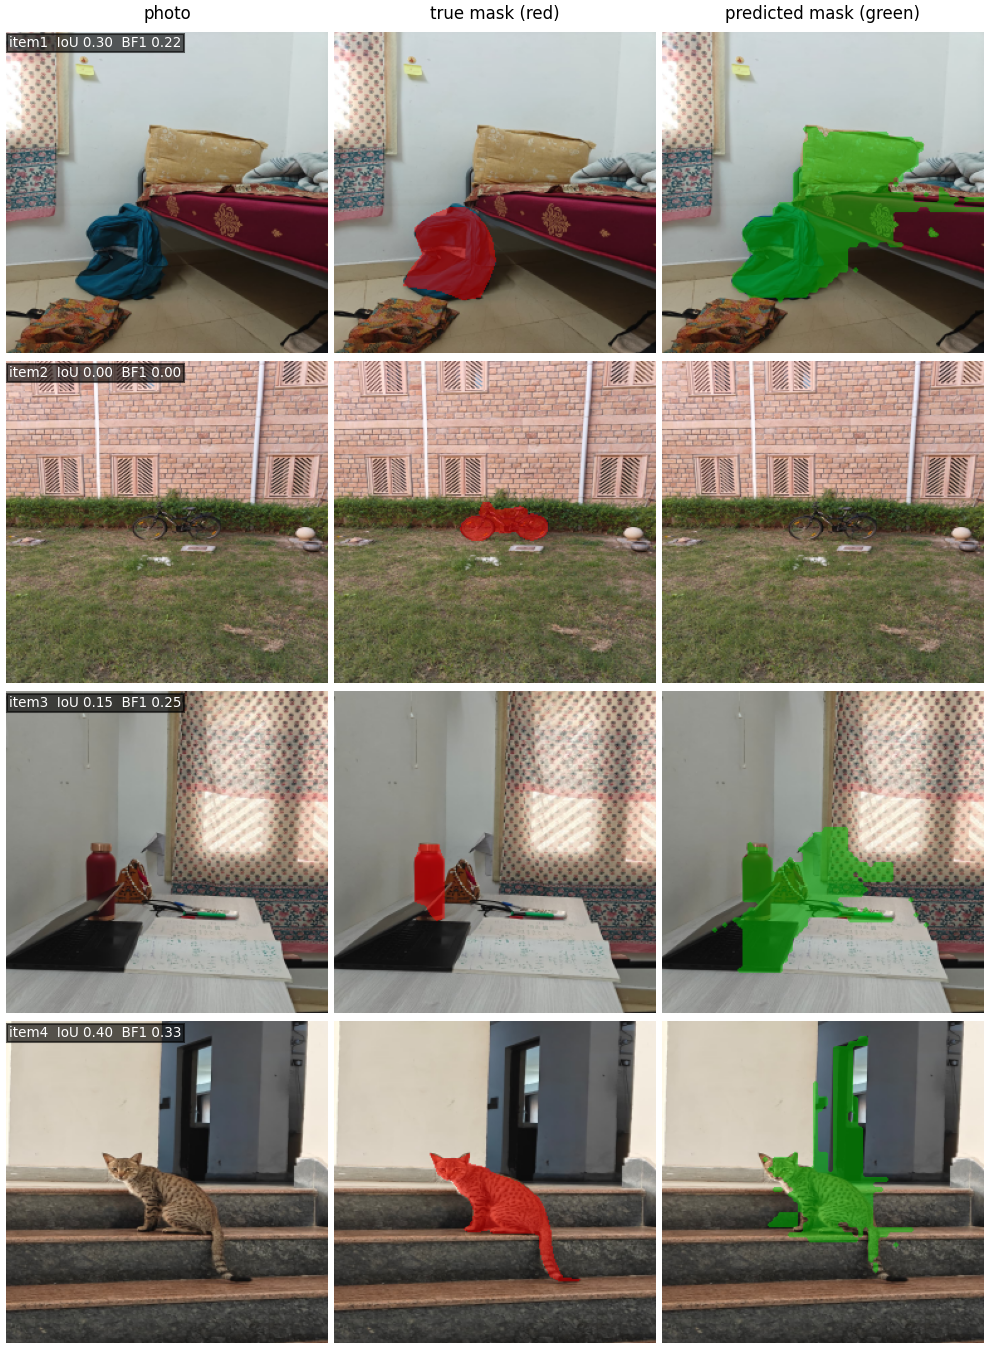
\includegraphics[width=\linewidth]{figures/captured_1.png}\caption{Captured photos, photo | true mask | predicted mask.}\label{fig:cap1}\end{figure}
\begin{figure}[h]\centering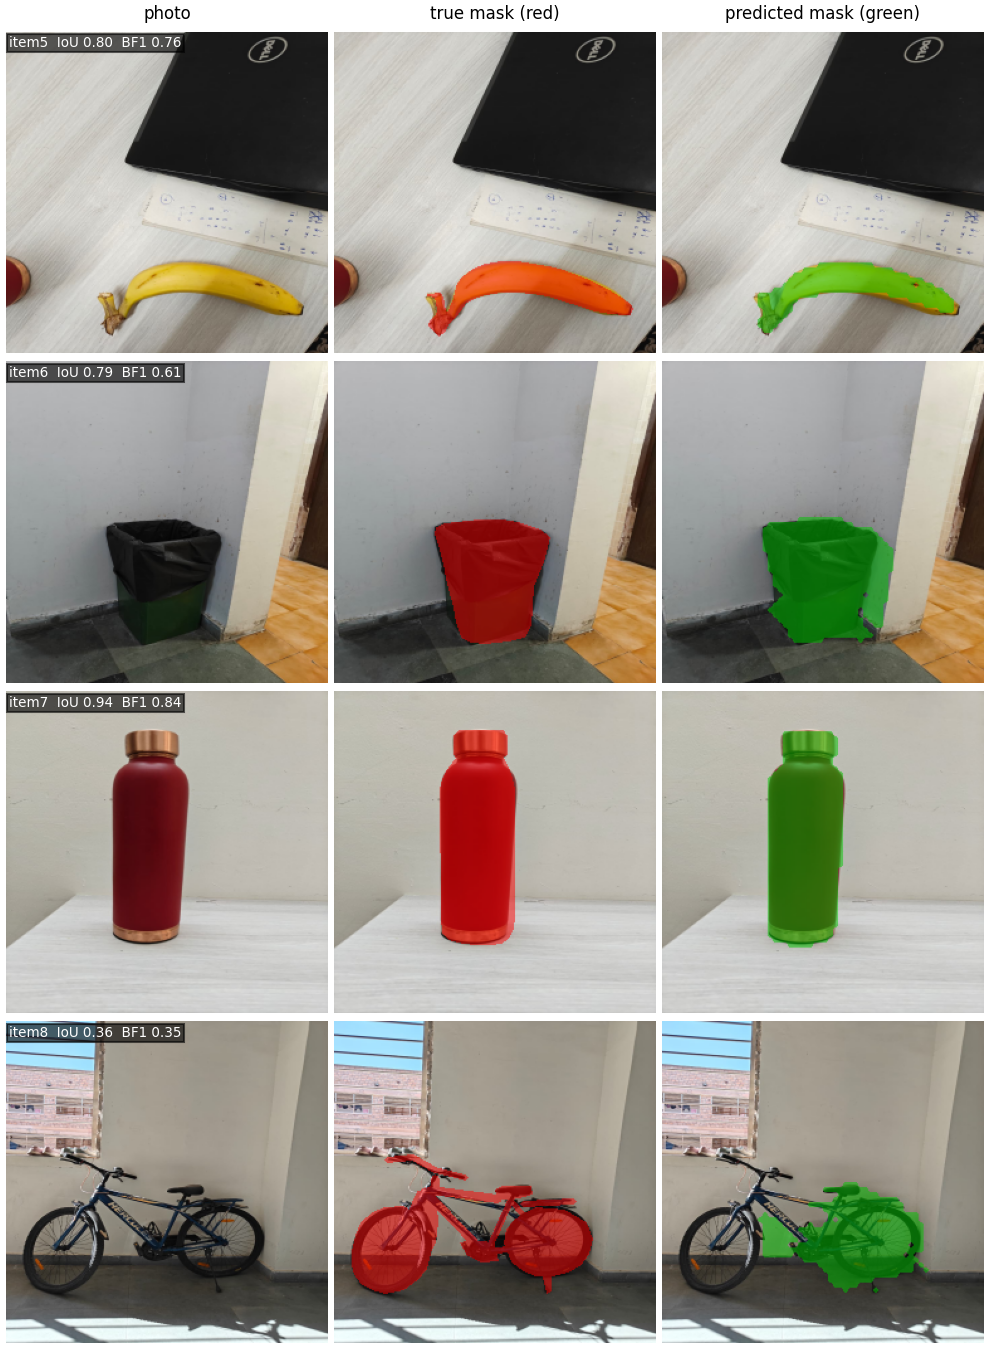
\includegraphics[width=\linewidth]{figures/captured_2.png}\caption{Captured photos, photo | true mask | predicted mask.}\label{fig:cap2}\end{figure}

\section{Failure cases}
Figure~\ref{fig:tefail} shows four DUTS-TE failures. Selection: 12 photos were drawn at random (seed 0) from the 1707 TE photos with IoU $<0.25$, and four of the draw were chosen because each shows a different kind of failure. They are examples, not a ranking of the worst cases.
\begin{figure}[h]\centering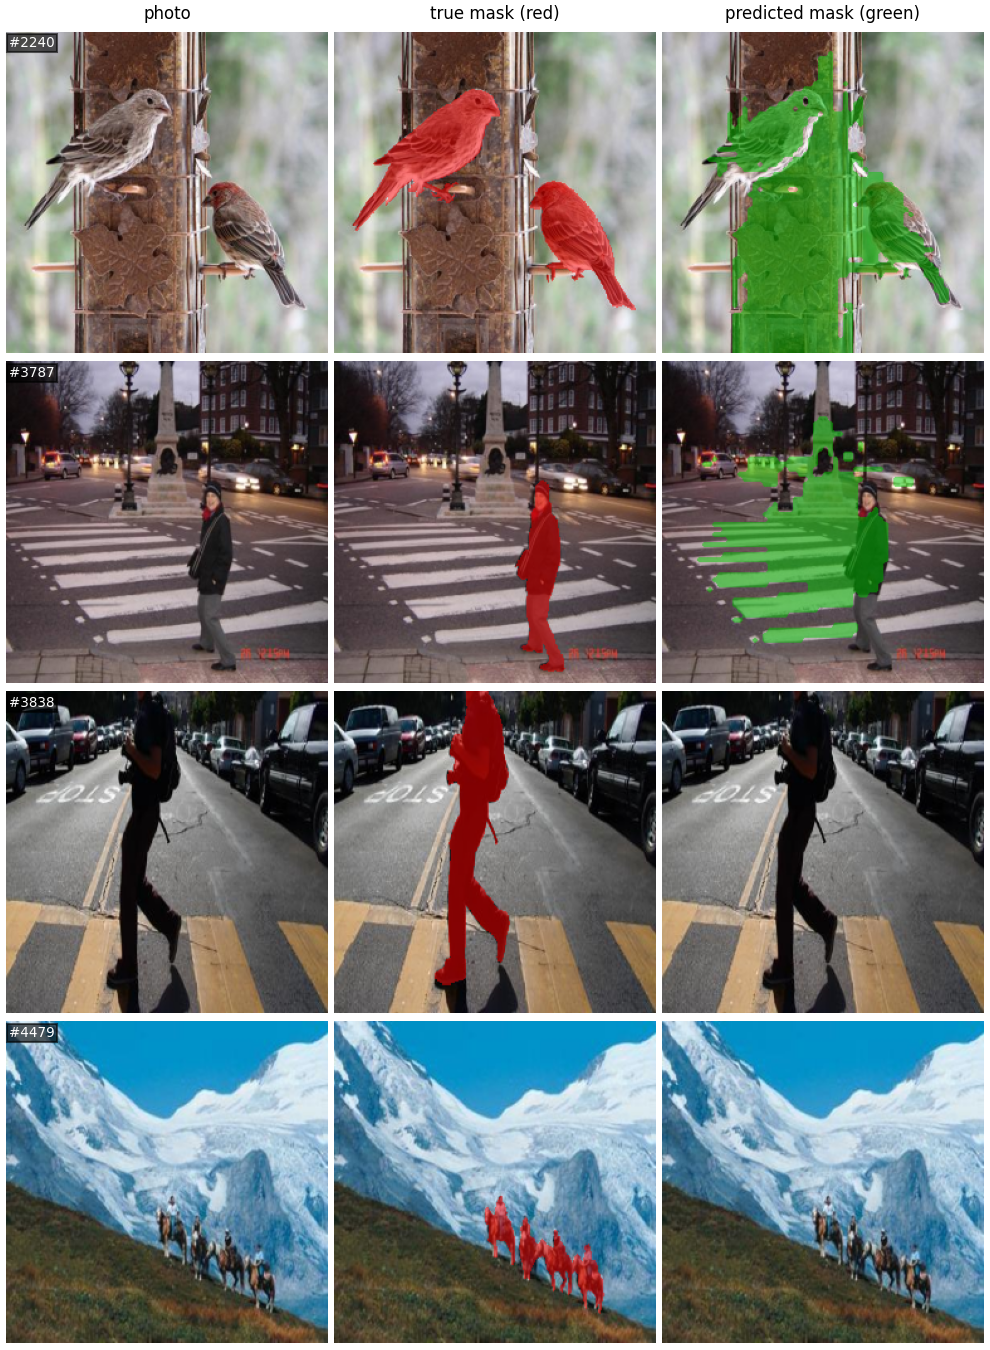
\includegraphics[width=\linewidth]{figures/te_failures.png}
\caption{DUTS-TE failures (photo | true mask | predicted mask).}\label{fig:tefail}\end{figure}
\begin{itemize}\itemsep0pt
\item \textbf{\#2240} -- textured distractor: the feeder is labelled object instead of (most of) the birds.
\item \textbf{\#3787} -- high-contrast distractor: the pedestrian is found, but zebra-crossing stripes and part of the monument are added.
\item \textbf{\#3838} -- poor light: dark backlit figure on a dark road, nothing predicted.
\item \textbf{\#4479} -- small object: the riders cover only 3.7\% of the photo, nothing predicted.
\end{itemize}
\textbf{Likely causes.} The region model only sees region-level colour, position, contrast and sharpness statistics (these causes are my interpretation of the examples, not separately tested). (1)~\emph{Small objects} are covered by only a few of the 144 regions (a region is about $5{\times}5$ pixels of the $64{\times}64$ image), so a single wrong region or a missed region
costs most of the object; the position prior and the pairwise smoothing, both learned/tuned on DUTS-TR where objects are large, probably also favour large central blobs (object IoU 0.15 below 2\% area vs 0.47 for 10--40\%). (2)~\emph{Clutter and strong
background contrast}: contrast and sharpness cues probably fire on the textured or high-contrast background (feeder, zebra crossing), which looks more salient to the region model than the true object. (3)~\emph{Poor lighting}: a silhouette whose colour is
close to the dark road has little colour contrast, so the colour-based cues are uninformative and the border-contact cues vote for background. (4)~\emph{Thin or see-through structures} cannot be captured at $64{\times}64$.
\paragraph{Captured photos.} Results are very uneven ($Q=0.626$ overall, per-photo object IoU from 0.00 to 0.94, Table~\ref{tab:cap}); with eight photos, this overall number is dominated by a few easy cases and should not be read
as better or worse generalisation than DUTS-TE. The three easy cases (item5 banana, item6 dustbin, item7 bottle) are large, saturated or high-contrast objects on a plain, low-texture background,
which is what the colour-contrast and border-contact cues of the model reward. The weakest photos (item2, item3, item1; Figure~\ref{fig:capfail}) are:
\begin{itemize}\itemsep0pt
\item \textbf{item2} (far bicycle, 2.1\%, IoU 0): nothing is predicted. It is a small, dark, thin structure (spoked wheels, tubes) in front of a dark hedge: low colour contrast, only a handful of the 144 regions, and a $64{\times}64$ working resolution that cannot represent the spokes.
\item \textbf{item3} (red bottle behind the laptop lid, IoU 0.15): the bottle is found, but the laptop lid, the ornament and the curtain are added to it. The occluding laptop lid is a large dark region next to the bottle with a similar contrast, and the model has no notion of an object being behind another.
\item \textbf{item1} (backpack, IoU 0.30): the bag is found, but the pillow and part of the mattress are added: the neighbouring pillow is more saturated and contrasty than the teal bag, and regions of similar colour are merged by the graph cut.
\end{itemize}
Two further photos are partial successes: in item8 (bicycle in hard sunlight) only the middle part of the bicycle is found and the front wheel and handlebar are missed (thin tubes, spokes and shadow patterns on the floor), and in item4 (cat) the body is found but the tail is missed and parts of the door frame and step edges are added.
These explanations are my reading of the figures and were not tested separately.
\begin{figure}[h]\centering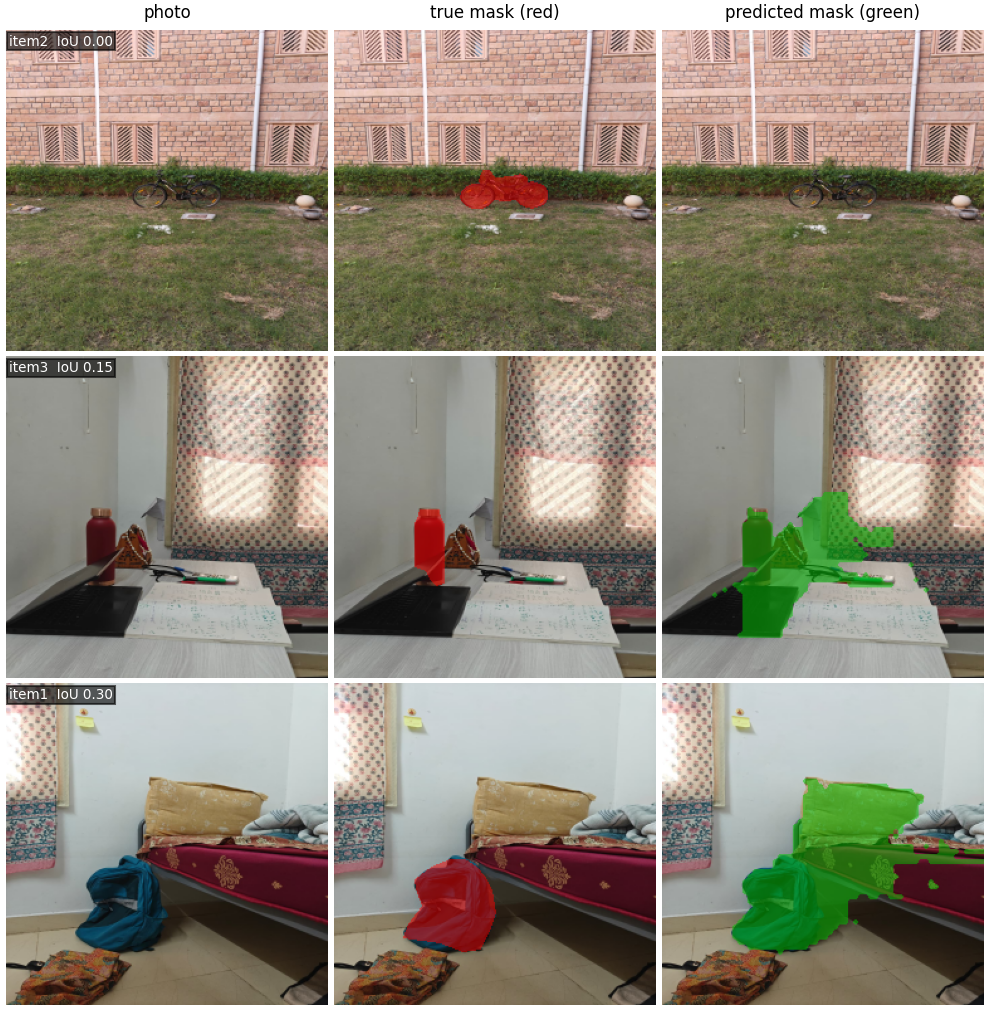
\includegraphics[width=\linewidth]{figures/captured_failures.png}
\caption{The three captured photos with the lowest object IoU.}\label{fig:capfail}\end{figure}

\paragraph{Limitations.} The approach has no notion of objects or semantics: it can only use colour, position, contrast and focus statistics of $\approx$144 regions, and it was fitted to DUTS-TR, whose objects are larger than those of DUTS-TE.

\end{document}
